% !TEX root=/home/tavant/these/manuscript/src/manuscript.tex




\chapter{Parametric study of the dielectric characteristics}
\label{ch-2}
Structure :

{\bf II. Parametric study of the dielectric} 30 pages
\begin{zzz}
  This chapter takes the 1rst paper which uses Vivien's results.

  2.1 Fully metallic wall (no SEE, grounded).

  2.2 Impact of Dielectric layer without SEE

  2.3 Impact of SEE with grounded wall

  2.4 SEE and dielectric in the same time

  2.5 Discrepancy between $\mean{\Te}$, $\sigma_{PIC}$ and $\sigma_{theo} = \sigma_0 + (1 - \sigma_0) \frac{2 T_e}{\epsilon_0}$
\end{zzz}

As introduced in \Cref{ch-1}, the \ac{HET} behaviour is dependent of the axial electron transport toward the anode across the magnetic barrier.
Two main phenomena are proposed to enhance the electron mobility,
\begin{itemize}
  \item the azimuthal instability \ac{ECDI}
  \item the electron emission
\end{itemize}
In order to compare quantitatively the relative importance of the two phenomena, we propose to conduct a parametric study on the dielectric wall characteristics.

As highlighted, the \ac{ECDI} rises due to the $E \times B$ electron drift, but saturate thanks to the axial convection model.
Before investigating the time dependent behaviour of the system, we focus in this \Cref{ch-2} on the average values at steady state.
The first section describe the parameters of the simulation, 
while the second section highlight the main characteristics of the simulation result.


% !TEX root=/home/tavant/these/manuscript/src/manuscript.tex

\section{Simulation parameters}
  \label{sec-params}
  
  The simulation domain corresponds to the exit plane of the thruster.
  Hence, a neutral pressure $P_n$ of 0.1~mTorr and a plasma density $n_e$ of $\sn{1}{17}$ m$^{-3}$ are used.
  The fixed axial electric field and radial magnetic field are $E_z=\sn{2}{4}\,\volt\per\meter$ s and $B_r=200$ G, respectively.
  The rectangular \ac{2D} domain measures $L_r=2$~cm in the radial dimension and $L_{\theta}=0.5$~cm in the azimuthal direction.
  The axial length used for the convection is fixed at $L_z=1$~cm.
  It is important to note that the results shown in this chapter have been obtained at the beginning of my thesis, before the study of the convection presented in \cref{ch-1}.
  Hence, in this chapter we use the convection model of \citet{lafleur2016a}.
  However, we have validated at posteriori that the convection model used does not modify the results under the conditions studied.
  
  The numerical parameters are chosen to respect the stability criterion of \ac{PIC} simulation, and are presented in \Cref{parameters}
  
  \begin{table}[htbp] %PIC parameters
       \centering
       \ra{1.3}
       \caption{\label{parameters} Standard operating and numerical parameters used in the 2D PIC simulations of an HET.  The simulation results are given as representative values.}
       \begin{tabular}{@{}r c c c@{}} 
          \toprule
          {\bf Physical Parameter} & notation & Value & Unit \\
          \midrule
          Gas & & Xenon & - \\
          Domain dimensions & $L_{x} \times L_{y} \times L_{z}$ & $2.0 \times 0.5 \times 1.0$ & [cm$^3$] \\
          Radial magnetic field & $B_{0}$                    & $200$                 & [{G}] \\
          Axial electric field & $E_{0}$                    & $2 \times 10^{4}$     & [{Vm}$^{-1}$] \\
          Mean plasma density & $n_{0}$                    & $3 \times 10^{17}$    & [{m}$^{-3}$] \\
          Initial electron temperature & $\Te_{,0}  $               & $5.0$                 & [{V}] \\
          Initial ion temperature & $T_{i,0}   $               & $0.1$                 & [{V}] \\
          Secondary electron temperature & $T_{see}   $               & $1.0$                 & [{V}] \\
          Neutral gas pressure & $P_{n}     $               & $1.0$                 & [{mTorr}] \\
          Neutral gas temperature & $T_{n}     $               & $300$                 & [{K}] \\
          Neutral gas density & $n_{g}     $               & $3.22 \times 10^{19}$ & [{m}$^{-3}$]\\
          \midrule
          {\bf Simulation Parameter} &  &   &  \\
          
          Time step & $\Delta t  $                      & $4 \times 10^{-12}$ & [{s}] \\
          Cell size & $\Delta x = \Delta y = \Delta z $ & $2 \times 10^{-5}$  & [{m}] \\
          Number of particles per cell & $N/NG      $                      & $80$                & [{part/cell}] \\
          \midrule
          {\bf Typical quantities} &  &  &  \\ 
          Electron plasma frequency & $\omega_{pe}$               & $3.1 \times 10^{10} $  & [rad/s]\\
          Iopn plasma frequency & $\omega_{pi}$               & $36 \times 10^{6} $  & [rad/s]\\
          Electron cyclotron frequency & $\omega_{ce}$               &  $3.5\times 10^{9}$  & [rad/s] \\
          Electron Larmor radius & $r_{Le}$                    & 6$\times 10^{-4}$    & [m] \\
          \bottomrule
       \end{tabular}
    \end{table}
  
  
  The simulation is initialized with a uniform density of particles, following a Maxwellian distribution for temperature $\Te_{,0}$ and $\Ti_{,0}$ for the electrons and the ions respectively.
  
  
% !TEX root=/home/tavant/these/manuscript/src/manuscript.tex

\section{The base case}
  \label{sec-canonical}
  
  
  The {\it base} case corresponds to the case when the walls are grounded, and are fully absorbing. 
  It is the reference case that will be extensively described and commented.
  Then, it will be used as reference to analyze and quantify the effects of two characteristics of the dielectric walls on the studied discharges : the secondary electron emission, and the modification of the electrostatic boundary condition.
  
  \subsection{Initial phase of the simulation\string: \texorpdfstring{$t < 2\,\micro\second$}{ t < 2 microseconds} } \label{subsec-initlaphase}
  
  The initial phase of the simulation corresponds to the growth of the \ac{ECDI}, and the formation of the sheaths.
  Because of the growth of the instability, the electron transport increases as well, which increases the electron heating.
  The time scale of the sheath formation is governed by the ion inertia.
  It is roughly the same time scale as the saturation of the instability due to ion-trapping.
  
  \begin{figure}[hbt]
    \centering
    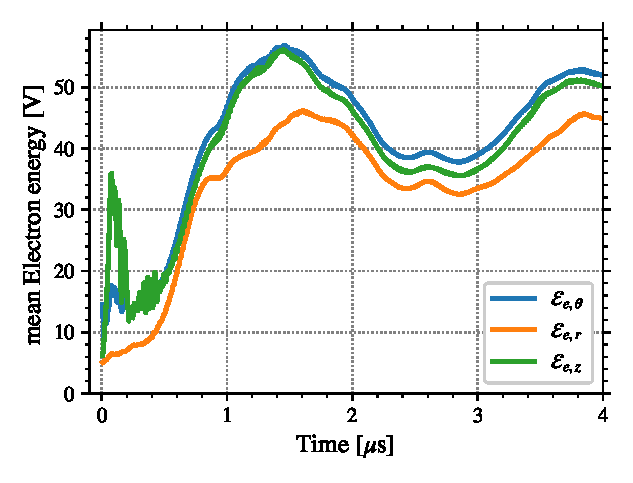
\includegraphics[width=\defaultwidth]{canonical_Te_start_directions}
    \caption{Temporal evolution of the electron mean kinetic energy decomposed over the three directions. Only the beginning of the simulation is shown.}
    \label{fig-canon_Te_strat}
  \end{figure}
  
  \Cref{fig-canon_Te_strat} shows the temporal evolution of the electron mean kinetic energy decomposed over the three directions, $\Ee_r, \Ee_{\theta}, \Ee_z$, such that
  \begin{equation} \label{eq-Ee_direction}
    \Ee_d = \frac{1}{n} \frac{1}{2} m_e \iiint_{\vect{v}}  v_{e,d}^2 f (\vect{v}) d^3v, \text{ with } d \in \{r, \theta, z  \}
  \end{equation}
  The mean kinetic energy is the sum of the thermal energy and the kinetic energy of the mean velocity.
  Because the electrons drift mainly in the azimuthal direction, we have
  \begin{equation} \label{eq-kinetic}
    \begin{cases}
      \Ee_r \simeq \frac{\Te_r}{2} \\
      \Ee_z \simeq \frac{\Te_z}{2} \\
      \Ee_{\theta} \simeq \frac{\Te_{\theta}}{2} + \frac{m_e}{2} \lp \frac{E_0}{B_0} \rp^2 \\
    \end{cases}
  \end{equation} 
  with $\frac{m_e}{2} \lp \frac{E_0}{B_0} \rp^2 \simeq  2.84\,\volt $.
  \nomenclature[Q]{\ensuremath{ \Ee}}{ Electron total kinetic energy, imposed of the thermal (or internal) energy and the kinetic energy of the mean velocity.  }
  We see that after some high frequency oscillations of $\Ee_{\theta}$ and $\Ee_z$ due to the cyclotron motion, the energies rise before stabilizing at $\Ee \simeq 45$V.
  The radial kinetic energy $\Ee_r$ is less than $\Ee_z$ and $\Ee_{\theta}$, but only by a small difference of $5\,\volt$, corresponding to roughly $10\%$.
  The small difference between the azimuthal and the axial kinetic energy is of the order of $2\,\volt$, as expected from the cyclotron motion of the electrons and \cref{eq-kinetic}.
  This means that the electrons are almost isotropic.
  
  
  \begin{figure}[hbt]
    \centering
    \begin{tabular}{@{} c c}
      \subfigure{time_r_mean_n}{a}{20, 20} &
          
      \subfigure{time_r_mean_phi}{b}{20, 20} 
    \end{tabular}
    \caption{Temporal evolution of the radial profile of the ({\bf a}) electron density and ({\bf b}) the plasma potential averaged azimuthally.}
    \label{fig-tx_n_phi}
  \end{figure}

  We can see in \Cref{fig-tx_n_phi} the evolution of the radial profile of the electron density on the plasma potential over the same period as \cref{fig-canon_Te_strat}.
  We observe on both quantities the formation of the sheath and the evolution toward a steady-state.
  
  \subsection{Saturated quasi steady-state\string: \texorpdfstring{$t \geq 2\,\micro\second$}{t > 2 microseconds}  }
  \label{subsec-stablephase}
  After the relatively fast rise of the plasma characteristics, the simulation reaches a quasi steady-state, as we can see in \Cref{fig-canon_Te_all}.
  We observe that after $t\simeq2\mus$ , the electron energy $\Ee$ starts to oscillate around a mean value.
  The oscillations are then damped and reach their minimum amplitude at  $t\simeq 7\mus$ and then remain with a small amplitude as shown on simulations carried out up to $25\,\micro\second$ in \cref{fig-canon_Te_all} (the origin of these oscillations has been discussed in \Cref{subsec-temp}).  
  
  
  \begin{figure}[hbt]
    \centering
    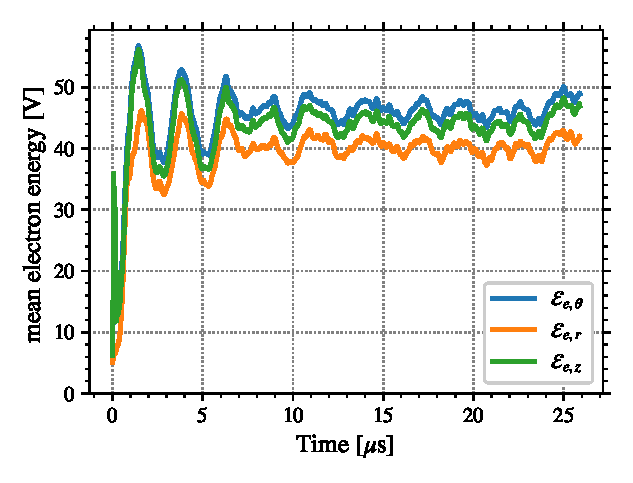
\includegraphics[width=\defaultwidth]{canonical_Te_all_directions_long}
    \caption{Temporal evolution of the electron mean kinetic energy decomposed over the three directions, similar to \cref{fig-canon_Te_strat} but for a longer period. We still see the difference between $\Ee_z$ and $\Ee_{\theta}$ due to the $E\times B$ drift, and the colder radial energy.}
    \label{fig-canon_Te_all}
  \end{figure}
  

  \Cref{fig-profiles} shows the azimuthally-averaged radial profiles of the electron and ion densities.
  The plasma is mostly quasineutral, except close to the walls, in the sheath, where the electron density falls more rapidly compared to that of ions.
  The sheath length can be roughly estimated to be $1\,\milli\meter$.
  The Debye length in our conditions is
  \begin{equation} \label{eq-debye}
    \lambda_D = \sqrt{\frac{\epsilon_0 k_b T_e}{n_e e^2}} \sim 0.4\,\milli\meter,
  \end{equation}
  which corresponds to the expected floating sheath length \citep{chabert2014} (a few $\lde$).
  
  \begin{figure}[hbt]
    \centering
    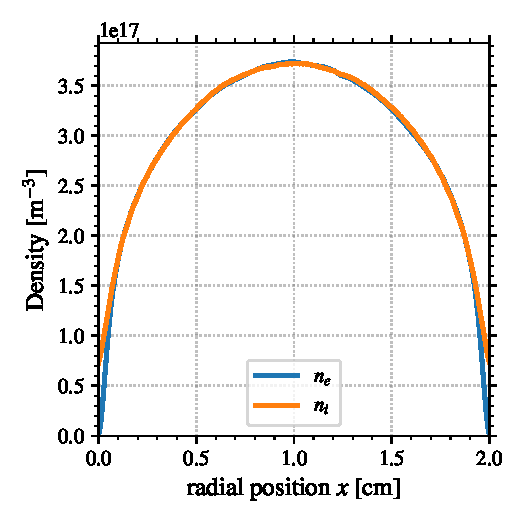
\includegraphics[width=\defaultwidth]{density_profile.pdf}
    \caption{Radial profile of the ion and electron densities at steady-state, averaged azimuthally and in time over the 5 last microseconds.}
    \label{fig-profiles}
  \end{figure}
  
  \subsection{Enhanced electron transport} \label{subsec-canonmue}
  As introduced in \cref{sec-transport}, the electron cross-field axial transport is characterized by the electron mobility
  \begin{equation} \label{eq-mobdef}
    \mob = \frac{u_{e, z}}{E_z}
  \end{equation}
  with $u_{e,z}$ and $E_z$ the electron mean axial velocity and the axial electric field, respectively.
  \nomenclature[Q]{\ensuremath{ \mob}}{ Electron mobility}
  \nomenclature[Q]{\ensuremath{ u}}{ Electron mean velocity}
  In \ac{PIC} simulations, $\mob$ is computed at each time step by
  \begin{equation} \label{eq-mobpic}
    \mobpic = \frac{1}{N E_z} \sum_N v_{e,z}
  \end{equation}

  \begin{figure}[hbt]
    \centering
    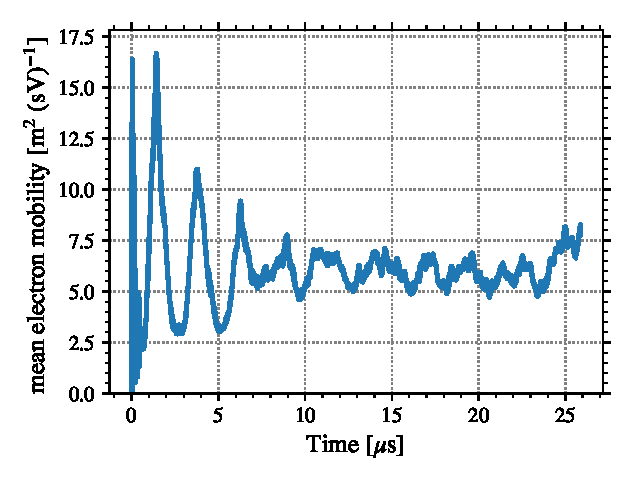
\includegraphics[width=\defaultwidth]{canonical_mu_all}
    \caption{Temporal evolution of the electron axial mobility computed in the \acs{PIC} simulation.}
    \label{fig-canon_mu}
  \end{figure}
  
  \Cref{fig-canon_mu} shows the temporal evolution of the electron mobility $\mobpic$ measured in the simulation with \cref{eq-mobpic}.
  We can see that it presents the same characteristics as the evolution of the electron energy $\Ee$ on \cref{fig-canon_Te_all}.
  We recall that the classical electron mobility from the collisional theory developed in \cref{eq-mobility} is \citep{lafleur2016a}
  \begin{equation} \label{eq-muclass}
    \mobcla = \frac{\nu_m \frac{e}{m_e}}{\oce^2 + \nu_m^2}
  \end{equation}
  with $\nu_m$ the electron-neutral  collision frequency and \oce{} is the electron cyclotron frequency.
  In the conditions of \cref{parameters}, $\mobcla \simeq 0.8$ \square\meter(sV)$^{-1}$.
  
  The measured electron mobility in the \ac{PIC} simulation is one order of magnitude larger than the classical mobility.
  In the present case, as no electron is emitted from the wall, the enhancement can only come from the instabilities present in the plasma.

  % K_ex = 2 10^-13
  % n_g = 1e19
  % wce = q B / m
  The oscillations can be seen in \cref{fig-2dschemat}, which shows the azimuthal electric field observed at $T=4\,\micro\second$.
  It clearly features the oscillation of wavelength of the order of 1~mm, as observed in \citet{heron2013}, and \citet{janhunen2018}.
  \Cref{fig-exampleECDI} shows the temporal evolution of the azimuthal electric field measured at the center of the channel.
  We can see that the instability rises and saturates quickly.
  Then, the oscillation remains quite stable.
  The Fourier Transform of the electric field presents a clear maximum at $14\,\mega\hertz$.
  The theoretical frequency of the \ac{ECDI} instability is \citep{lafleur2017}
  \begin{equation} \label{eq-maxfeq}
    f_{\rm max} = \frac{\omega_{pi}}{\sqrt{3}} \simeq 21 \,\mega\hertz,
  \end{equation}
  which gives a relatively good agreement with the oscillation observed.
  The \ac{ECDI} instability was the subject of \Cref{ch-5}, hence it will not be further discussed here.
  
  
  \begin{figure}[hbt]
    \centering
    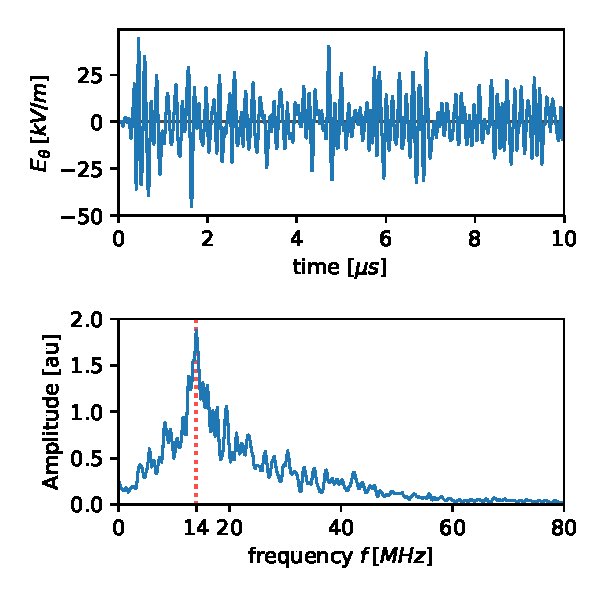
\includegraphics[width=\defaultwidth]{time_and_FFT}
    \caption{Azimuthal instability\string: temporal evolution of the azimuthal electric field at the center of the simulations, and its frequency spectrum computed by \acs{FFT}. The frequency for which the amplitude is maximum is highlighted.}
    \label{fig-exampleECDI}
  \end{figure}
  
  The effective mobility $\mobeff$ is determined by the correlation term $<\dEt \dne>$ and the parameters of the simulations.
  The effective mobility at saturation $\mobeffsat$, using the hypothesis of saturation by ion-wave trapping, only needs the electron temperature $\Te$.
  We can see that the three values $\mobpic, \mobeff$, and $\mobeffsat$ are close from each-others.
  
  \begin{table}[!hbt]
  \ra{1.3}
    \centering
    \caption{Characteristics  measured in the simulation at $t=27\,\micro\second$.}
    \label{tab-canonical_mobility}
    \begin{tabular}{@{} r l @{}} \toprule
    Quantity & Value \\ \midrule
    Correlation $<\dEt \dne>$ & $\sn{6}{20}$ V/m${^4}$ \\
    Effective mobility $\mobeff$ from \cref{eq-eq_mobeffsimple_two} & 4.4 m$^2$(sV)$^{-1}$ \\
    Mobility saturation $\mobeffsat$ from \cref{eq-mobeffsat} & 3.3 m$^2$(sV)$^{-1}$ \\
    Measured mobility $\mobpic$ from \cref{eq-mobpic} & 6 m$^2$(sV)$^{-1}$\\
    \bottomrule
    \end{tabular}
  \end{table}
  

  
  
% !TEX root=/home/tavant/these/manuscript/src/manuscript.tex

\section{Conclusion of the parametric study}
  \label{sec-conclusion_ch2}
  
  Using the \ac{PIC} simulation code introduced in \cref{ch-1}, we studied the effects of the dielectric walls on the discharge, and more precisely the effects on the electron axial mobility.
  To begin with, a \emph{base} case with metallic walls was defined and studied.
  The metallic walls correspond to grounded and non-emissive walls.
  For this reference case, we observed that the convection model used allows us to obtain a quasi steady-state.
  We observed an enhanced electron transport transverse to the magnetic field lines, because of the azimuthal instability.
  Both effects of the dielectric -- the electron induced electron emission and the electrostatic boundary condition -- were investigated.
  First, we  only modeled the dielectric boundary condition. Then, we studied only the electron emission. Afterwards, the two phenomena have been studied together.
  
  \subsubsection*{Electrostatic boundary condition}
  
  The electrostatic boundary condition is modeled by including in the domain of simulation the thickness of the wall ($L_{\rm Diel} = 3 \milli\meter$).
  Surface charges accumulate at the interface between the plasma and the wall.
  We observed that the modified boundary condition did not modify significantly the discharge and the axial cross-field electron mobility.
  Moreover, we saw that the boundary condition used results in a radial electric field $E_r$ of the same order of magnitude than the Neumann boundary condition of \cref{eq-neuman} but the spatio-temporal evolution is not identical.
  
  Indeed, when the secondary electron emission is modeled, the surface charges oscillates significantly compared to the radial electric field during the \ac{SCL} regime.
  As the dielectric model used here do not increase significantly the computational time, we recommend to use it instead of the Neumann boundary condition, that do not reproduce the same plasma-wall interaction.
  
  
  \subsubsection*{Electron induced electron emission}
  
  The electron  emission from the wall due to the impact of primary electron reaching the wall is modeled using the model described in \cref{sec-seemodel}.
  The value of the crossover energy $\crover$ is varied from a large value (low emissivity) to small values (high emissivity).
  We observed in the simulations that when the electron emission rate increases, the mean electron temperature decreases.
  This decreases the amplitude of the \ac{ECDI} at saturation, hence decreases the electron mobility in the plasma (see \cref{fig-radial-data}).
  However, electron emission induces \ac{NWC}, which almost doubles the electron mobility close to the wall when $\crover$ varies from $200\volt$ to $30\volt$.
  Consequently, the overall electron cross-field mobility is almost constant in our simulation.
  
  We observed in our \ac{PIC} simulations three different regimes depending on the values of $\crover$.
  For high values of $\crover$, the plasma stabilises with an emission rate $\ratepic < \ratecr$.
  When $\crover$ is small, we observe a stable configuration with $\ratepic \sim \ratecr$.
  Under these conditions, the sheath is space-charge limited.
  The transition between the two regimes is not stable, but instead passes by a bi-stable regime.
  In this third regime, the sheath jumps between the two stable regimes.
  

  \subsubsection*{Inconsistent sheath model }
  
  The simulation results have been compared to the sheath model of \citet{hobbs1967}.
  We observed a significant discrepancy between the \ac{PIC} simulations and the sheath model that comes from a fluid approach.
  In particular, the potential drop and the electron emission rate are both overestimated.
  These overestimations can lead to erroneous conclusion and prediction when using fluid models.
  Hence, a better understanding of the plasma-wall transition via the sheath is needed.
  
  The sheath model currently used is based mainly on two hypothesis
  \begin{itemize}
    \item Maxwellian electron distribution function
    \item Isothermal electrons in the sheath
  \end{itemize}
  
  Both hypotheses will be questioned in the next chapter.
  

